% $Id: template.tex 11 2007-04-03 22:25:53Z jpeltier $

\documentclass{vgtc}                          % final (conference style)
%\documentclass[review]{vgtc}                 % review
%\documentclass[widereview]{vgtc}             % wide-spaced review
%\documentclass[preprint]{vgtc}               % preprint
%\documentclass[electronic]{vgtc}             % electronic version

%% Uncomment one of the lines above depending on where your paper is
%% in the conference process. ``review'' and ``widereview'' are for review
%% submission, ``preprint'' is for pre-publication, and the final version
%% doesn't use a specific qualifier. Further, ``electronic'' includes
%% hyperreferences for more convenient online viewing.

%% Please use one of the ``review'' options in combination with the
%% assigned online id (see below) ONLY if your paper uses a double blind
%% review process. Some conferences, like IEEE Vis and InfoVis, have NOT
%% in the past.

%% Figures should be in CMYK or Grey scale format, otherwise, colour 
%% shifting may occur during the printing process.

%% These few lines make a distinction between latex and pdflatex calls and they
%% bring in essential packages for graphics and font handling.
%% Note that due to the \DeclareGraphicsExtensions{} call it is no longer necessary
%% to provide the the path and extension of a graphics file:
%% \includegraphics{diamondrule} is completely sufficient.
%%
\ifpdf%                                % if we use pdflatex
  \pdfoutput=1\relax                   % create PDFs from pdfLaTeX
  \pdfcompresslevel=9                  % PDF Compression
  \pdfoptionpdfminorversion=7          % create PDF 1.7
  \ExecuteOptions{pdftex}
  \usepackage{graphicx}                % allow us to embed graphics files
  \DeclareGraphicsExtensions{.pdf,.png,.jpg,.jpeg} % for pdflatex we expect .pdf, .png, or .jpg files
\else%                                 % else we use pure latex
  \ExecuteOptions{dvips}
  \usepackage{graphicx}                % allow us to embed graphics files
  \DeclareGraphicsExtensions{.eps}     % for pure latex we expect eps files
\fi%

%% it is recomended to use ``\autoref{sec:bla}'' instead of ``Fig.~\ref{sec:bla}''
\graphicspath{{figures/}{pictures/}{images/}{./}} % where to search for the images

\usepackage{microtype}                 % use micro-typography (slightly more compact, better to read)
\PassOptionsToPackage{warn}{textcomp}  % to address font issues with \textrightarrow
\usepackage{textcomp}                  % use better special symbols
\usepackage{mathptmx}                  % use matching math font
\usepackage{times}                     % we use Times as the main font
\renewcommand*\ttdefault{txtt}         % a nicer typewriter font
\usepackage{cite}                      % needed to automatically sort the references
\usepackage{tabu}                      % only used for the table example
\usepackage{booktabs}                  % only used for the table example
%% We encourage the use of mathptmx for consistent usage of times font
%% throughout the proceedings. However, if you encounter conflicts
%% with other math-related packages, you may want to disable it.


%% If you are submitting a paper to a conference for review with a double
%% blind reviewing process, please replace the value ``0'' below with your
%% OnlineID. Otherwise, you may safely leave it at ``0''.
\onlineid{0}

%% declare the category of your paper, only shown in review mode
\vgtccategory{Research}

%% allow for this line if you want the electronic option to work properly
\vgtcinsertpkg

%% In preprint mode you may define your own headline.
%\preprinttext{To appear in an IEEE VGTC sponsored conference.}

%% Paper title.

\title{Notification preferences based of of location and location activities}

%% This is how authors are specified in the conference style

%% Author and Affiliation (single author).
%%\author{Roy G. Biv\thanks{e-mail: roy.g.biv@aol.com}}
%%\affiliation{\scriptsize Allied Widgets Research}

%% Author and Affiliation (multiple authors with single affiliations).
%%\author{Roy G. Biv\thanks{e-mail: roy.g.biv@aol.com} %
%%\and Ed Grimley\thanks{e-mail:ed.grimley@aol.com} %
%%\and Martha Stewart\thanks{e-mail:martha.stewart@marthastewart.com}}
%%\affiliation{\scriptsize Martha Stewart Enterprises \\ Microsoft Research}

%% Author and Affiliation (multiple authors with multiple affiliations)
\author{Tri Nguyen\thanks{e-mail:Tri95182}\\ %
     \parbox{1.4in}{\scriptsize \centering Colorado State University \\ Computer Science\\ CS464:HCI}}

%% A teaser figure can be included as follows, but is not recommended since
%% the space is now taken up by a full width abstract.
%\teaser{
%  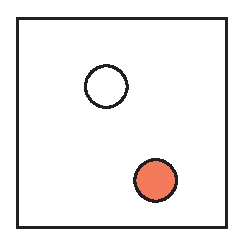
\includegraphics[width=1.5in]{sample.eps}
%  \caption{Lookit! Lookit!}
%}

%% Abstract section.
\abstract{Most Americans own smartphones nowadays, about 97\% says the Pew research center, this is a big change over the last decade compared to 35\% when the Pew first started back in 2011. With this rise in smartphones is also a rise in many users experiencing stress from receiving notifications all the time. In this paper we will be looking into the users of smartphones and their relationship between notifications and stress. Specifically this paper's goal is to better understand that relationship within the variable of location. In order to understand that, I collected a small set of data about where people most often are, in their day, between home and some type of work or school activity. I used snapchat and my own app created with android studio, to record surveys of my users. This allowed us to better understand some users' preferences on when they should receive notifications in terms of location. This small survey study can show users preferences for receiving notifications at certain locations.%
} % end of abstract

%% ACM Computing Classification System (CCS). 
%% See <http://www.acm.org/class/1998/> for details.
%% The ``\CCScat'' command takes four arguments.

\CCScatlist{ 
Notification; smartphone; stress; interruption;
messenger app 

}

%% Copyright space is enabled by default as required by guidelines.
%% It is disabled by the 'review' option or via the following command:
% \nocopyrightspace

%%%%%%%%%%%%%%%%%%%%%%%%%%%%%%%%%%%%%%%%%%%%%%%%%%%%%%%%%%%%%%%%
%%%%%%%%%%%%%%%%%%%%%% START OF THE PAPER %%%%%%%%%%%%%%%%%%%%%%
%%%%%%%%%%%%%%%%%%%%%%%%%%%%%%%%%%%%%%%%%%%%%%%%%%%%%%%%%%%%%%%%%

\begin{document}

%% The ``\maketitle'' command must be the first command after the
%% ``\begin{document}'' command. It prepares and prints the title block.

%% the only exception to this rule is the \firstsection command
\firstsection{Introduction}

\maketitle

%% \section{Introduction} %for journal use above \firstsection{..} instead
Since the beginning of technology, especially heading into the industrial era we have used alarms to alert us of certain situations within our tech environments. As we continue evolving with the technology around us we still use alarms to interact with it. Through notifications, we interact with many of the applications that we use daily, from phone notifications to daily reminders. This allows companies to alert us when we need to pay attention or if anything in the app got updated that we might want to check. Because this tool is so useful to companies to increase interaction it brings the question of how to most effectively send notifications so that the notification has high engagement. 
What I mean in high engagement is users opening the app and interacting with it. Doing this while trying to make sure to not annoy the user. Allows for higher engagement in the app.[6] 
The interaction of notifications works on several contextual factors such as the smartphone position, the user’s location, and their activity [1]. In this paper I will be looking into the factor of user’s location and investigate the preferences of my participants for different notification modals.
The content types of using smartphone notifications include messenger messages, SMSs, phone calls, mail services, social network services, games, advertisements, system states, update alerts, etc. Smartphones offer various methods for receiving notifications, including a status bar, LED indicator, screen pop-up, vibration, sound, or a combination of these in order to let a user know that he or she has received a notification 
Found in other literature pushes a correlation between a user’s location and the activity performed at that location aka “location-based activity”.[2] Location information will be collected in 2 formats, GPS and Location-based activity. GPS location can be correlated with Google maps, to find the building they are located in. The location-based activity will be collected via survey when the user opens the notification. In this paper we will investigate the user’s locations effects on participants notification’s receptivity and interruptibility [4&5]


\section{Related Works}
In this paper the goal is to better understand notification perception through understanding users' annoyance levels and activity interruption as well as users' relationship to stress and notifications. If we look at current studies done there are signs that show that increased push notifications stresses the users.[9] My goal is to isolate the variable of locations and to better understand stresses of push notifications based on location. To do that we need to also examine associated works in the domains of receptivity and interruptibility detection, specifically on mobile phones. There is plenty of related work that looks into breaking points and activity changes[6]. These papers show that the moment to send a notification is when the user is switching from one task to another, it showed that during this moment in time that it would increase user receptivity[7]. These papers show that there is a high chance or correlation between tasks and receptivity.
	Also studies done in the mobile app space have shown that there is a coloration between frequency of push notifications and user open rate[11]. The correlation shows that after a certain point pushing to many notifications can be bad. 
Park et al. concluded that users do not want to be interrupted while being socially engaged [5]. The Social context is an area of land that is related to the user in which for itself can play a variable in a user's interruptibility. Social context, activity, and location were considered together in a set of features used for interruptibility detection.[3] Due to their extensive consideration in literature, we will focus on location and location-based activities and investigate their influence on a user’s perception of notifications. 
All these studies relate how receptive a user is to those notifications, and with much of the location based research based off of location activity over just home or work, I wanted to do this study to see if maybe we can simplify the experiment to understand if it's the activity or the location itself. 

\section{Methodology}
The goal in this paper is to get a first impression about preferences for notifications modal based on location, specifically for mobile notifications.I’ve decided to run this in a more natural setting, using peoples phones, and a survey. I had 10 users participate in this study, it is a within-subject as we have users test both sides of receiving notifications. The goal is to observe my participants and how they interact with notifications if they know when they receive the notification based on location.
\subsection{Design}
 My study will mostly have my participants be within-subjects, as each participant marks their ‘Home’ and ‘Work/School’ location and we send randomly timed notifications when the user is located within these areas. I will send these notifications out at around 15 minutes after entering the marked locations. Upon receiving the notification, a timer will start to see how long it takes for the participant to open the notification, along with how long it takes to fill out the survey. Which will consist of questions similar to other studies[3]:
\item
How Unpleasant was the reception of this notification(1-not,7-Very Unpleasant)
\item
How interruptive was this notification in general(1-not,7-Very interruptive)
\item
What activities did this notification interrupt feel free to list a few(short answer)
\item
How interruptive was this notification to that particular activity(1-not,7-Very interruptive)
\section{Prototype}
Before I got into the study methods, Originally I had planned to make an app with Push Notifications and GPS tracking but the SQL and Google API wasn’t working the way I wanted to. Specifally I had issues using intergrating pusher beams and channels to do push notfications. Also I couldn't track user 24/7 with the survey library I was using. In the video that I show of my app you can see that it is the full survey and I get the users locations. Then it records that into a file onto the phone. The problem is that I needed the users' locations before sending the survey. So I could know when they are home or at work before sending the survey. Also only 4 out of the 10 of my willing participants had an android phone. So In realization that I wanted more subjects and didn’t necessarily need to create an app I changed the app into 2 different methods, Snapchat and Google survey. This allows me a lot more flexibility in who can participate in my survey. A image of the google survey can be see in figure 1

\begin{figure}
 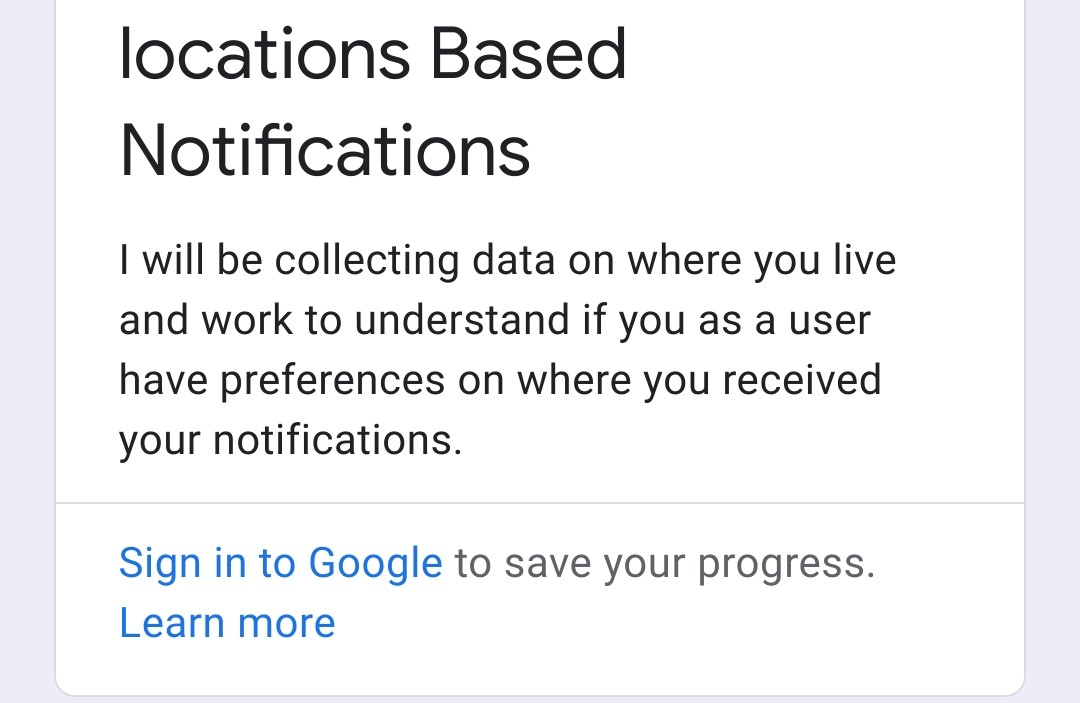
\includegraphics[width=\columnwidth]{Survey1.jpg}
 \caption{This is a taste of what my google survey looked like}
 \label{fig:sample}
\end{figure}

\begin{figure}
 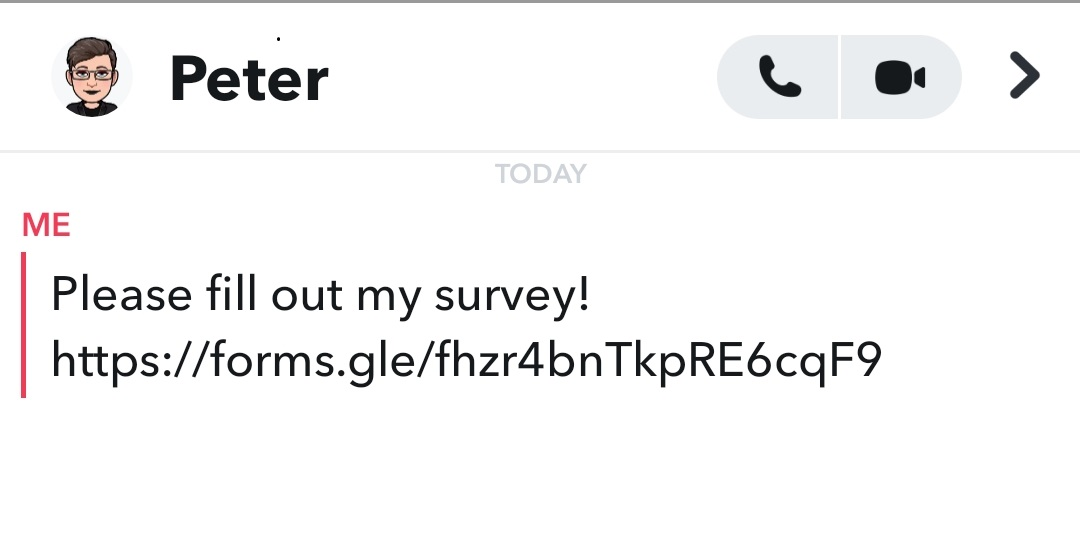
\includegraphics[width=\columnwidth]{Snap.jpg}
 \caption{This is a sending my snap notification looked like}
 \label{fig:sample}
\end{figure}

\begin{figure}
 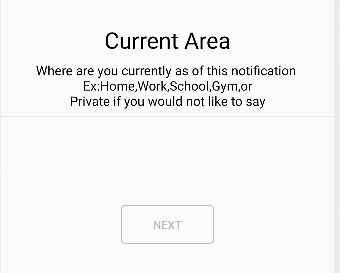
\includegraphics[width=\columnwidth]{OldApp.png}
 \caption{This is a what my survey app looked like}
 \label{fig:sample}
\end{figure}

\section{Experiment}
I had 10 users participate in this study, it is a within-subject as we have users test both sides of receiving notifications. This was a 3 day study first day was presurvey, then day 2 was running the survey and day 3 was interviewing the subjects to understand there data better.
\subsection{Pre-survey}
In the Pre-survey, I asked for the users consent to collect private data then. I collected my users, names,Snap Username, home addresses, work(or school) address) and what device they were using.Also if they spend more time at school or work.I also made sure that they accepted me on snap at that time and made sure that there snap location tracking was on at least for me. I only send notifications to whichever they spent more time in as school and work are similar in tasks. This allowed me to know when people were home or at school based on if they were near these addresses. 
\subsection{Survey Day}
During the Survey day, I would note who’s bitmojis I’m tracing on snapchat then send a msg to fill out my survey when I noticed they were home. Or at work. The survey was very simple all it asked was to\item
How Unpleasant was the reception of this notification(1-not,7-Very Unpleasant)\item
How interruptive was this notification in general(1-not,7-Very interruptive)\item
What activities did this notification interrupt feel free to list a few(short answer)\item
How interruptive was this notification to that particular activity(1-not,7-Very interruptive)

This was done twice that day, 1 time for home, 1 time for work, the timing was random. I would check snapmaps every 1 hour or so, so within an hour of most people arriving at work or home they received a message from me to fill out a survey. Doing this gave me 10 surveys per location type. 
\subsection{Exit Survey}
On the last day I asked the users to tell me where they would prefer to receive locations and why. Many of the answer revealed that most people were busy at work and had more free time at home. This shows more clearly in my data later. 
\section{Survey Results}

Let's get this out there first. This survey is based on ten people so the results should be verified with a bigger pool to be accurate. But based on my survey, receiving messages at home or at work is similarly annoying. Home Being 4.9 and Work being 5.4 on a scale from 1 to 7. This is very close and I think shows that the app and work you're doing on the app affects the annoyance more than the location. But for Interruptive there is a clear lower average for home than for work, this is more abundant when you look at the differences in tasks and Task Interruptibility. Most people's Work tasks were more involved than home this led to a very high activity interrupted number. This number represents how much the notifications interrupting that activity and that was 3.9 - Home vs 6 - Work/School. It is clear in table 1, for this one day that most people working didn't not like to be interrupted to fill out a survey. It was useful in asking how interruptive the notification was in general vs the activity. 


 This also true when I asked each user their preferences for receiving notifications the next day.  With most users preferring to receive notifications at home over work. On a scale of 1 being I like notifications at home vs 7 being you like notifications at work. The average came out to 6. When I asked for their reasoning most answered along the lines of I’m busy at school/work, which I guess makes sense, we go to school/work to get things done and are usually busy. When Looking closer at the data it is pretty clear that many of the activities that my subject is doing at work would be more involved and harder to do then many of the ones they do at home. 
It seems that there is a huge coloration between activity and notifications interaction. 

\subsection{Conclusion}

In general this data set is too small to really be conclusive about my results. But if I were to take my data at its word its aligns with many of the other papers I’ve read where location is important but only because of the type of activities you should expect to do there, When doing this experiment it seemed that home was better place to receive notifications because it was less interruptive to the activities at hand. While on the opposite spectrum work/school was more interruptive to the task at hand. When reading the activity vs the interruptions it was clear that if people were doing easier activities at work then they would be more receptive to notifications or harder tasks at home less receptive.So It really had less to do with the location but more to do with the activity. It just so happens that the activities you do at home are usually less intense then the ones you do at work.


\begin{table}[tb]
  \caption{Averages from the data(1-low,7-high).}
  \label{tab:vis_papers}
  \scriptsize%
	\centering%
  \begin{tabular}{|l|l|l|l|}
\hline
Location & Annoyed & Interruptive & Interruptive Activity \\ \hline
Work AVG    & 5.4                 & 4.9                  & 6                            \\ \hline
Home AVG     & 4.9                 & 3                    & 3.9                          \\ \hline
\end{tabular}
\end{table}



%% if specified like this the section will be committed in review mode
\acknowledgments{
The authors wish to thank A, B, C. This work was supported in part by
a grant from XYZ.}

%\bibliographystyle{abbrv}
\bibliographystyle{abbrv-doi}
%\bibliographystyle{abbrv-doi-narrow}
%\bibliographystyle{abbrv-doi-hyperref}
%\bibliographystyle{abbrv-doi-hyperref-narrow}

\bibliography{template}
Sunny Consolvo and Miriam Walker. 2003. Using the experience sampling method to evaluate ubicomp applications. IEEE Pervasive Computing 2, 2 (2003), 24–31.

 Exler, Anja, et al. “Preferred Notification Modalities Depending on the Location and the Location-Based Activity.” Adjunct Proceedings of the 2019 ACM International Joint Conference on Pervasive and Ubiquitous Computing and Proceedings of the 2019 ACM International Symposium on Wearable Computers, 2019, https://doi.org/10.1145/3341162.3344842. 
 
 Anja Exler, Marcel Braith, Andrea Schankin, and Michael Beigl. 2016. Preliminary investigations about interruptibility of smartphone users at specific place types. In UbiComp’16 Adjunct. ACM, 1590–1595.

Chunjong Park, Junsung Lim, Juho Kim, Sung-Ju Lee, and Dongman Lee. 2017. Don’t Bother Me. I’m Socializing!: A Breakpoint-Based Smartphone Notification System. In CSCW’17. ACM, 541–554 

Mikio Obuchi, Wataru Sasaki, Tadashi Okoshi, Jin Nakazawa, and Hideyuki Tokuda. 2016. Investigating interruptibility at activity breakpoints using smartphone activity recognition api. In PUbiComp’16 Adjunct. ACM, 1602–1607.

Joel E Fischer, Chris Greenhalgh, and Steve Benford. 2011. Investigating episodes of mobile phone activity as indicators of opportune moments to deliver notifications. In MobileHCI’13. ACM, 181–190.

Anja Exler, Marcel Braith, Kristina Mincheva, Andrea Schankin, and Michael Beigl. 2018. Smartphone-Based Estimation of a User Being in Company or Alone Based on Place, Time, and Activity. In MobiCase’18. Springer, 74–89. 

SungHyuk Yoon, Sang-su Lee, Jae-myung Lee, and KunPyo Lee. 2014. Understanding notification stress of smartphone messenger app. In CHI '14 Extended Abstracts on Human Factors in Computing Systems (CHI EA '14). Association for Computing Machinery, New York, NY, USA, 1735–1740. https://doi.org/10.1145/2559206.2581167

Swaan C, van den Broek A, Kretzschmar M, Richardus JH. Timeliness of notification systems for infectious diseases: A systematic literature review. PLoS One. 2018 Jun 14;13(6):e0198845. doi: 10.1371/journal.pone.0198845. PMID: 29902216; PMCID: PMC6002046.

Atilla Wohllebe, Dirk-Siegfried Hübner, Uwe Radtke and Szilárd Podruzsik (2021). Mobile apps in retail: Effect of push notification frequency on app user behavior. Innovative Marketing , 17(2), 102-111. doi:10.21511/im.17(2).2021.10

\end{document}
